\subsubsection{Dashboard - Estad�stica de consumo de electricidad por sector}
En el primer tab, ``Consumo``, tenemos una estad�stica de consumo por grupo de consumidores de energ�a. Al abrir este panel, observamos que la el grupo de consumidores residencial es la que m�s demanda energ�a, hist�ricamente. Otro dato interesante es la exportaci�n de energ�a el�ctrica, que seg�n el gr�fico, cada vez fue disminuyendo m�s. 
A nivel nacional la zona residencial se ubica en primer lugar con un 39,87\%.  Luego viene el sector industrial, que consume el 22.11\% de la energ�a. El sector comercial es due�a del 17,39\%.


\textsc{\begin{figure}[H]
	\centering
	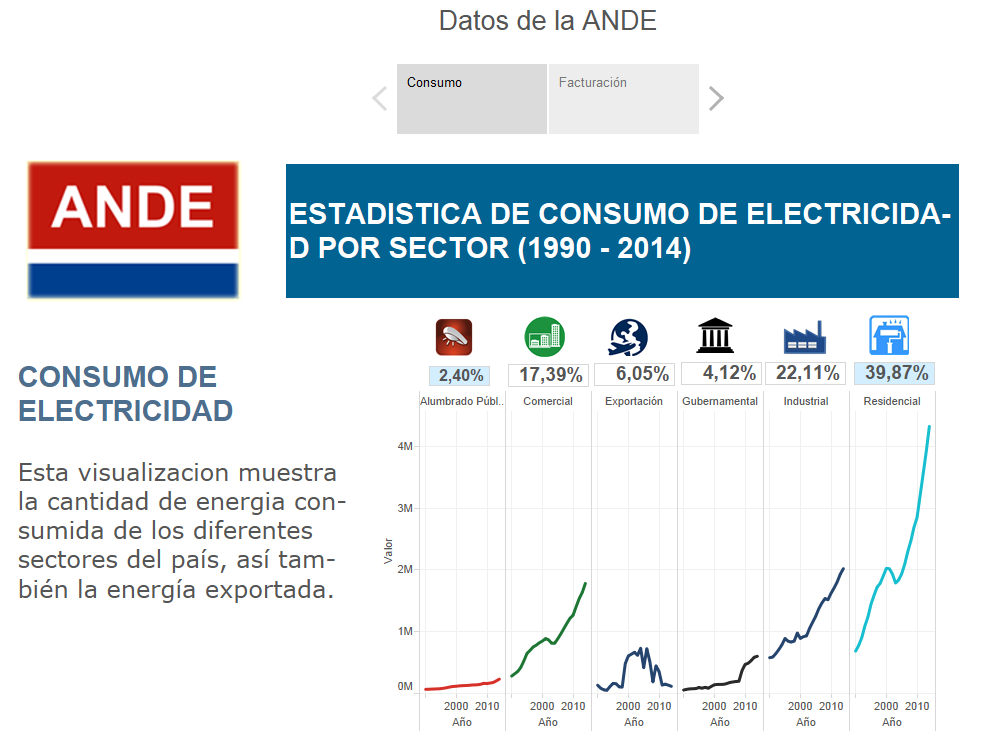
\includegraphics[width=\linewidth]{figuras/EstadisticaDeConsumoDeElectricidadPorSector1990-2014}
	\caption{Estad�stica de consumo de electricidad por sector(1990-2014)}
	\label{fig:EstadisticaDeConsumoDeElectricidadPorSector1990-2014}
\end{figure}}

En el segundo tab, titulado ``Facturaci�n``, tenemos datos de facturaciones por grupo de consumidores.  Al igual que el gr�fico anterior observamos que la zona residencial es a la que m�s facturas se emiten.


\textsc{\begin{figure}[H]
	\centering
	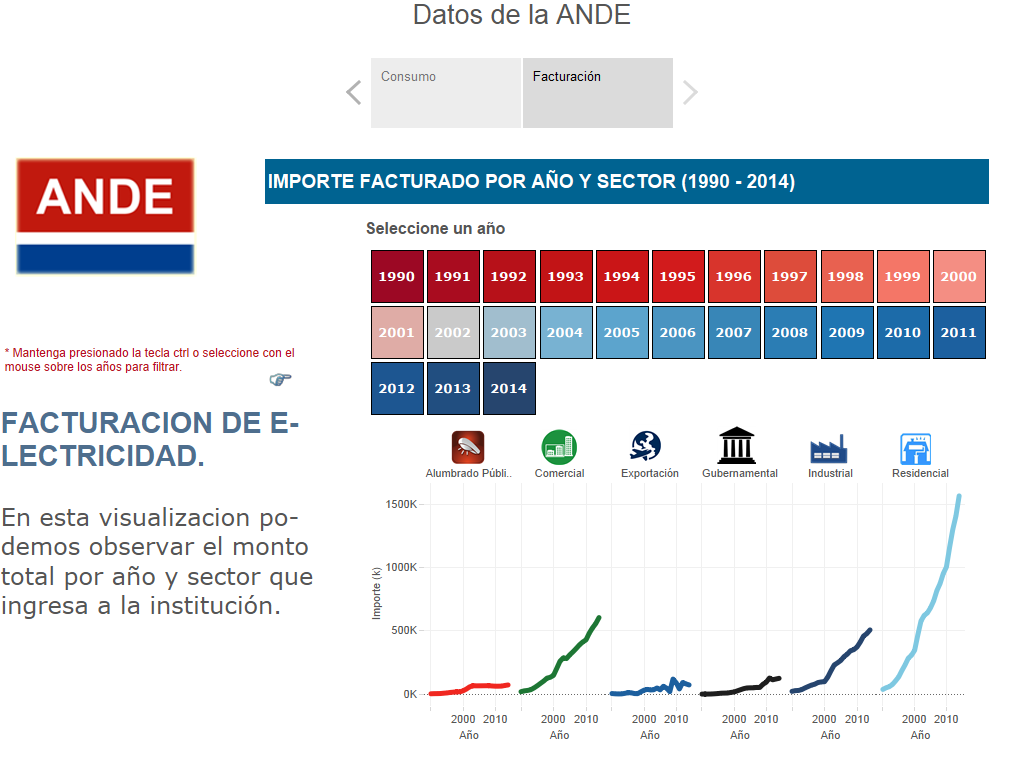
\includegraphics[width=\linewidth]{figuras/ImporteFacturadoPorAnoYSector1990-2014}
	\caption{Importe facturado por a�o y sector(1990-2014)}
	\label{fig:ImporteFacturadoPorAnoYSector1990-2014}
\end{figure}}